\documentclass{beamer}

\usepackage{beamerthemesplit}
\usepackage{graphicx}
\usepackage{color, natbib, hyperref}

%theme

\usetheme{boxes} 
%\usecolortheme{seahorse} 
\setbeamertemplate{items}[default] 
%\setbeamercovered{transparent}
\setbeamertemplate{blocks}[rounded][shadow=true] 
\setbeamertemplate{navigation symbols}{} 

\mode<presentation>

\title[SET]{Student Evaluations of Teaching (Mostly) Do Not Measure Teaching Effectiveness}
\author{Kellie Ottoboni}
\institute[]{Department of Statistics, UC Berkeley \\ Berkeley Institute for Data Science}
\date{May 3, 2016}

\begin{document}

\frame{\titlepage}

\section{Introduction}


\frame{
\frametitle{~}
  \begin{columns}[T]
    \begin{column}{.5\textwidth}
    \begin{center}
    
\includegraphics[width=0.8\textwidth]{headshot/pbs.jpg} \\
    Philip B. Stark \\
    UC Berkeley
    \end{center}
    \end{column}
    \begin{column}{.5\textwidth}
    \begin{center}
    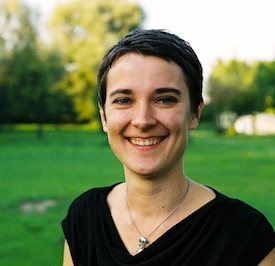
\includegraphics[width=0.8\textwidth]{headshot/AnneBoring.jpg} \\
    Anne Boring \\
    SciencesPo University
    \end{center}
    \end{column}
  \end{columns}
}

\frame
{
  \frametitle{ ~}
 \begin{center}
 \Large{ Student evaluations of teachers (SET) are used to} \\
  \begin{itemize}
  \item Quantify teaching effectiveness
  \item Compare instructors across courses
  \item Make hiring, firing, and promotion decisions  
  \end{itemize}
  \vfill
Are SET a valid measure of teaching effectiveness?
\end{center}
}

\frame
{
  \frametitle{ ~}
  \begin{center}
  \Huge{No!}
  \end{center}

\vfill
\Large
%  \begin{itemize}
%  \item SET measure ``customer satisfaction''
%  \item Ratings are biased against female instructors
%  \item Biases are inconsistent across universities and disciplines; impossible to ``adjust'' SET
%  \end{itemize}


We reanalyzed data from two studies: 
\begin{itemize}
\item a natural experiment in France (\cite{Boring2015})
\item a randomized experiment in the US (\cite{MacNell2014})
\end{itemize}


}

\section{The Data}
\frame
{
  \frametitle{Data from \cite{Boring2015}}
\begin{columns}[T]
\begin{column}{.5\textwidth}
\begin{center}
\begin{itemize}
\item Census of SET by first-year undergraduates, collected 2008--2013
\item Students sign up for class times, don't know instructors; it's ``as if'' at random
\item Male instructors are rated higher by male students than by female students
\item SET correlate with grade expectations but not final grades
\end{itemize}
\end{center}
\end{column}
\begin{column}{.5\textwidth}
% figures
\end{column}
\end{columns}

}


\frame
{
  \frametitle{Data from \cite{MacNell2014}}
\begin{columns}[T]
\begin{column}{.5\textwidth}
\begin{center}

\begin{itemize}
\item Students randomized to 4 online sections of a course
\item In two sections, the TAs swapped identities
\item Female-identified TA was rated lower on average in all categories
\end{itemize}
\end{center}
\end{column}
\begin{column}{.5\textwidth}
\begin{table}
\begin{tabular}{r|c}
\textbf{Characteristic} & \textbf{F - M} \\
\hline
Overall & -0.47 \\
Caring & -0.52 \\
Consistent & -0.47 \\
Enthusiastic & -0.57 \\
Fair & -0.76 \\
Feedback & -0.47 \\
Helpful & -0.46 \\
Knowledgeable & -0.35 \\
Praise & -0.67 \\
Professional & -0.61 \\
Prompt & -0.80 \\
Respectful & -0.61 \\
Responsive & -0.22
\end{tabular}
\end{table}
\end{column}
\end{columns}
}



\section{Analysis}
\frame
{
 \frametitle{Permutation tests}
\Large
 \begin{itemize}
 \item Distribution-free tests, always give correct significance levels
 \item Compare assumptions:
 \begin{itemize}
 \item Two-sample t-test: independent samples from normal distribution
 \item Permutation test: randomization was fair
 \end{itemize}
 \item{Python package: permute \\
 \url{https://github.com/statlab/permute}
 }
 \end{itemize}

}

\section{References}
\begin{frame}
\frametitle{References}
\bibliographystyle{plainnat}
\bibliography{SETs}
\itemize
\end{frame}
\end{document}
